% This is a LaTeX template for an ICSC submission, based on a homework template by Lucas R. Ximenes (Jimeens)
% Refactored for Dario Loi, M.Sc Computer Science, Sapienza University of Rome

%%%%%%%%%%%%%%%%%%%%%%%%%%%%%%%%%%%%%%%%%%%%%%%%%%%%%%%%%%%%%%%%%

\documentclass{solutionclass} % Using the original class as requested
\usepackage{listings} % Add the listings package for code highlighting
\usepackage{xcolor} % Required for defining custom colors
\usepackage{tikz} % Added for drawing neural network components
\usepackage{cleveref}
\usepackage{microtype}
\usepackage{hyperref}

% Define a custom Python style for the code listing
\lstdefinestyle{pythonstyle}{
    language=Python,
    backgroundcolor=\color{gray!10},
    commentstyle=\color{blue!30!black},
    keywordstyle=\color{red!75!black},
    numberstyle=\tiny\color{gray},
    stringstyle=\color{green!40!black},
    basicstyle=\ttfamily\footnotesize,
    breakatwhitespace=false,
    breaklines=true,
    captionpos=b,
    keepspaces=true,
    numbers=left,
    numbersep=5pt,
    showspaces=false,
    showstringspaces=false,
    showtabs=false,
    tabsize=2
}


\pagestyle{plain}

\begin{document}

\pretitle%
{ICSC 2025 Submission}                          % ⟸ Main Title
{Solutions to the Qualification Round}          % ⟸ Subtitle
{Dario Loi} % ⟸ Author and Affiliation

\makeatletter
    \startcontents[sections]
    \phantomsection%
    \chapter{Solutions}
\makeatother

    This document presents the solutions for the qualification round of the International Computer Science Competition (ICSC) 2025. Each section corresponds to a problem from the problem sheet. For programming problems, the source code is provided with a description and in-line comments, as per the submission guidelines.

    Student: Dario Loi\\
    \divider%

    \section{Problem A:\@ Neural Network Components}
    This section provides the identification and description of the neural network components as requested in Problem A.

    \begin{solution}[Solution to Problem A]
        \begin{tabular}{p{3cm} p{11cm}}
            % --- w_21^(1) ---
            \Large{$\textcolor{blue}{w^{(1)}_{21}:}$} & Weight multiplying input feature 2 (Tip received) and feeding into hidden feature 1.
            \vspace{0.7cm} \\
            
            % --- Sigma ---
            \Large{$\textcolor{orange}{\Sigma:}$} & Summation of all incoming weighted features, aggregates all of the contributions of the input features as a linear combination, before it's fed to the activation function $f$.
            \vspace{0.7cm} \\
            
            % --- f ---
            \Large{$\textcolor{cyan}{f:}$} & Activation Function (typically ReLU:\@ $f(x)=\max(0,x)$, historically sigmoid: $f(x)=\frac{1}{1+e^{-x}}$), ensures that the network can compute non-linear functions, allowing it to act as a universal approximator (according to the Universal Approximation Theorem).
            \vspace{0.7cm} \\

            % --- Input Neuron (Red Circle) ---
            
\begin{tikzpicture}\node[circle, draw=red, thick, fill=red!10, minimum size=8mm] {};\end{tikzpicture} : & Input Neuron, receives raw input features (in this case Duration Stayed and Tip Received) and passes them to the first hidden layer in a fully-connected fashion.
            \vspace{0.7cm} \\

            % --- Bias Neuron (orange Circle) ---
            
\begin{tikzpicture}\node[circle, draw=orange, thick, fill=orange!10, minimum size=8mm] {};\end{tikzpicture} : & Bias, a scalar summed to the linear combination of incoming features to ensure that the linear projection computed by the neuron is not constrained to pass through the origin.
            \vspace{0.7cm} \\

            % --- Output Neuron (Green Circle) ---
            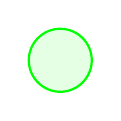
\begin{tikzpicture}\node[circle, draw=green, thick, fill=green!10, minimum size=8mm] {};\end{tikzpicture} : & Output Neuron, outputs final prediction $\hat{y}$.
            \vspace{0.7cm} \\

            % --- Box A ---
            \large{Box A:} & Hidden Layer, where the input features are transformed through weighted connections and non-linear activation functions to create higher-level representations.
            \vspace{0.7cm} \\
            
            % --- Box B ---
            \large{Box B:} & Output Layer, where the final predictions are made based on the transformed features from the hidden layer. \\
            \vspace{0.7cm} \\

            % --- y-hat ---
            \Large{$\hat{y}:$} & Final prediction: the probability of a restaurant customer being satisfied with their visit. Since $\hat{y}$ is a probability and $f$ is the same across the MLP, it is likely that $f(x)=\frac{1}{1+e^{-x}}$ (sigmoid function) is used, which outputs values in the range $[0, 1]$. \\ \\

        \end{tabular}
    \end{solution}

    \divider%

    \section{Problem B:\@ Cake Calculator}



    \begin{solution}[Source Code: CakeCalculator]
    This section provides the implementation of the \texttt{CakeCalculator} as requested in Problem B. We provide a $O(1)$ solution that directly calculates the required quantities without need for a \texttt{while} loop.

    \begin{lstlisting}[style=pythonstyle]
    from typing import Tuple

    def cake_calculator(flour: int, sugar: int) -> list:
        """
        Calculates the maximum number of cakes that can be made and the leftover ingredients.
        
        Args:
            flour: An integer larger than 0 specifying the amount of available flour.
            sugar: An integer larger than 0 specifying the amount of available sugar.
            
        Returns:
            A list of three integers: 
            [0] the number of cakes that can be made
            [1] the amount of leftover flour
            [2] the amount of leftover sugar
            
        Raises:
            ValueError: If inputs flour or sugar are not positive.
        """
        FLOUR_NEEDED = 100
        SUGAR_NEEDED = 50

        # This ensures robustness of our solution to invalid inputs, 
        # as our type hint only specifies "int"
        assert flour >= 0 and sugar >= 0, "Flour and sugar must be non-negative."

        # We use integer division (//) to calculate the maximum number of cakes
        # we can bake given the available flour and sugar.
        # We then take the min to ensure we don't exceed either ingredient.
        cakes = min(flour // FLOUR_NEEDED, sugar // SUGAR_NEEDED)

        # We calculate the spare amount of each ingredient by subtracting
        # the amount we actually used
        spare_flour = flour - (cakes * FLOUR_NEEDED)
        spare_sugar = sugar - (cakes * SUGAR_NEEDED)

        return cakes, spare_flour, spare_sugar
    \end{lstlisting}
    \end{solution}

    \divider%

    \section{Problem C:\@ School Messaging App}

    In this section, we answer the various questions about the information-theory related problem C.

    \begin{solution}[Question 1]
        As our message traffic analysis show, natural language messages do not exhibit a uniform distribution across their character set, rather, they tend to use some characters more frequently than others.

        Given a character set of size $N$, and a probability distribution $P(c)$ over the characters, we can define the expected length of a character in bits as:

        \begin{equation}\label{eq:exp_length}
            L = \sum_{c \in C} P(c) \cdot \text{size}(c)
        \end{equation}

        This formula captures the intuition that more frequent characters (higher $P(c)$) and larger characters (higher $\text{size}(c)$) contribute more to the expected length.

        To design an efficient encoding scheme, we should aim to assign shorter codes to more frequent characters and longer codes to less frequent characters, decreasing this expected value as much as possible.
    \end{solution}

    \begin{solution}[Question 2]
        We are then tasked to calculate the entropy for our 12-character set, which is defined as:

        \[
        H = -\sum_{c \in C} P(c) \log_2 P(c)
        \]

        We recall our character set to be:

        \vspace{0.5cm}

        \begin{center}
        \begin{tabular}{|c c|c c|}
            \hline
            Character & Probability $P(c)$ & Character & Probability $P(c)$ \\
            \hline
            A & $0.20$ & G & $0.05$ \\
            B & $0.15$ & H & $0.05$ \\
            C & $0.12$ & I & $0.04$ \\
            D & $0.10$ & J & $0.03$ \\
            E & $0.08$ & K & $0.02$ \\
            F & $0.06$ & L & $0.10$ \\
            \hline
        \end{tabular}
    \end{center}

        \vspace{0.5cm}

        Therefore we can calculate our entropy to be:

        \begin{align*}
            H &= -\sum_{c \in C} P(c) \log_2 P(c) \\
              &= -\Big( 
                    0.20 \log_2 0.20 
                  + 0.15 \log_2 0.15 
                  + 0.12 \log_2 0.12 \\
              &\qquad
                  + 0.10 \log_2 0.10 
                  + 0.08 \log_2 0.08 
                  + 0.06 \log_2 0.06 \\
              &\qquad
                  + 0.05 \log_2 0.05 
                  + 0.05 \log_2 0.05
                  + 0.04 \log_2 0.04 \\
              &\qquad
                  + 0.03 \log_2 0.03 
                  + 0.02 \log_2 0.02 
                  + 0.10 \log_2 0.10 
                \Big)\\
            &\approx 3.324
        \end{align*}

        This corresponds to the theoretical lower bound for the expected number of \emph{bits} needed to encode a message using this character set, assuming optimal encoding.

        This means that, no matter how efficient, no coding scheme can exist that achieves a lower average code length than $3.324$.
    \end{solution}

    \begin{solution}[Question 3]
        We calculate the average code length of the provided Fano encoding according to \Cref{eq:exp_length}. First we recall our Fano Code:

        \vspace{0.5cm}

        \begin{tabular}{|c c c|c c c|}
            \hline
            Character & Probability $P(c)$ & Fano Code & Character & Probability $P(c)$ & Fano Code \\
            \hline
            A & $0.20$ & $000$ & G & $0.05$ & $001$ \\
            B & $0.15$ & $100$ & H & $0.05$ & $1011$ \\
            C & $0.12$ & $010$ & I & $0.04$ & $0111$ \\
            D & $0.10$ & $1100$ & J & $0.03$ & $1101$ \\
            E & $0.08$ & $0110$ & K & $0.02$ & $1111$ \\
            F & $0.06$ & $1010$ & L & $0.10$ & $1110$ \\
            \hline
        \end{tabular}

        \vspace{0.5cm}

        We can now calculate the average code length of this Fano encoding using \Cref{eq:exp_length}:

        \begin{align*}
            L &= \sum_{c \in C} P(c) \cdot \text{size}(c) \\
              &= 
                0.20 \cdot 3 
              + 0.15 \cdot 3 
              + 0.12 \cdot 3 \\
            &\qquad
              + 0.10 \cdot 4 
              + 0.08 \cdot 4 
              + 0.06 \cdot 4 \\
            &\qquad
              + 0.05 \cdot 3 
              + 0.05 \cdot 4 
              + 0.04 \cdot 4 \\
            &\qquad
              + 0.03 \cdot 4 
              + 0.02 \cdot 4 
              + 0.10 \cdot 4 \\
            &\approx 3.480
        \end{align*}

        Indeed the provided solution is quite efficient. We can calculate the efficiency of the encoding as follows:

        \begin{align*}
            \eta &= \frac{H}{L} \\
                 &\approx \frac{3.324}{3.480} \\
                 &\approx 0.955
        \end{align*}

        Meaning that our average message length under Fano encoding is $95.5\%$ close to the theoretical lower bound.

    \end{solution}

    \divider

    \section{Problem D: Word Choice Puzzle}
    \begin{solution}[Word Choice Puzzle description \& source code]
        The fourth question asks us to provide a code that generates a $10\times 10$ word choice puzzle. We attempt 
        to do this in the most creative way possible, by implementing these optional features:

        \begin{itemize}
            \item Given a set of words $W$, we generate a set of distractors $\hat{W}$ by removing the last character of each word in $W$, we only do this for words longer than $4$ letters to ensure that the resulting distractor can be picked up by the human eye, we also discard any distractors that would make $|\hat{W}| > 3$.
            \item We maximize intersections of legitimate words and distractors, creating a dense mesh of words that make it trickier for the user to find the correct words. We do so by scanning every grid cell in three possible directions (horizontal, vertical and diagonal).
            \item We fill the rest of the grid randomly. To prevent these random letters from turning a distractor into a copy of a full word accidentally, we temporarily mark cells with lowercase letters to indicate that that letter should be excluded from the generation process.
        \end{itemize}

        % Define helper macros (scoped locally inside this environment)
        {\renewcommand{\arraystretch}{1.15}%
        \newcommand{\wrd}[1]{\colorbox{yellow!60}{\strut\textbf{#1}}}% target word letter
        \newcommand{\di}[1]{\colorbox{red!65}{\strut\color{white}#1}}% distractor

        Below is an example of a $10 \times 10$ grid generated by our algorithm, reproducible by setting seet to $42$. We color target words and distractors for easy readability.
        
        
        notice how distractors \emph{can} overlap with completed words, meaning that letters belonging to a distractor can also be part of a full word, when this happens, we color that letter in yellow (full word takes priority).

        \medskip
        \centering
        \setlength{\tabcolsep}{3pt}
        \begin{tabular}{*{10}{c}}
            % Row 1
            \wrd{L} & \di{O} & \di{V} & \di{E} & \di{L} & \di{A} & \di{C} & \wrd{I} & P & J \\
            % Row 2
            \wrd{O} & Q & R & \wrd{E} & D & M & \di{O} & \wrd{C} & M & O \\
            % Row 3
            \wrd{V} & R & J & \wrd{N} & S & R & \di{M} & \wrd{S} & H & I \\
            % Row 4
            \wrd{E} & E & W & \wrd{T} & U & Q & \di{P} & \wrd{C} & I & Z \\
            % Row 5 (TURING)
            \wrd{L} & \di{T} & \di{U} & \wrd{R} & \di{I} & \di{N} & \di{U} & \wrd{T} & M & V \\
            % Row 6
            \wrd{A} & Y & Q & \wrd{O} & H & Z & \di{T} & \wrd{U} & T & *P \\
            % Row 7 (COMPUTER)
            \wrd{C} & \wrd{O} & \wrd{M} & \wrd{P} & \wrd{U} & \wrd{T} & \wrd{E} & \wrd{R} & T & H \\
            % Row 8
            \wrd{E} & W & M & \wrd{Y} & C & E & D & \wrd{I} & G & Q \\
            % Row 9 (extended)
            F & G & X & T & W & K & D & \wrd{N} & O & Z \\
            % Row 10 (extended)
            F & K & J & I & N & J & B & \wrd{G} & B & Y \\
        \end{tabular}

        \medskip
        \noindent\textbf{Legend:} \wrd{A} = letter belonging to one of the target words (ICSC, TURING, LOVELACE, COMPUTER, ENTROPY);\\ \di{A} = letter belonging to a distractor.

        \medskip

        Below we list the full source code for the Word Choice Puzzle generator, this is 
        quite long and will end up being typeset across multiple pages. For a more readable 
        version, check out the attached python file \texttt{problem\_d.py}.
        
\medskip

        \begin{lstlisting}[style=pythonstyle]
    def create_crossword(words: list) -> list:
        """
        Generate a 10x10 word search puzzle containing the given words.
        
        Args:
            words: A list of words to include in the puzzle.
            
        Returns:
            A 2D array (list of lists) representing the word search puzzle.
        """
        
        import string
        random.seed(42)
        
        # WRITE YOUR CODE HERE
        GRID_SIZE = 10
        base = [w.upper() for w in words]
        # generate distractors by removing the last character of each word longer than 4 letters
        # we only want at most 3 distractors
        distractors = [w[:-1].upper() for w in base if len(w) > 4][:3]
        full_map = {
            d: [f for f in base if f.startswith(d) and len(f) == len(d) + 1]
            for d in distractors
        }  # map distractor to its full word
        seq = sorted(base + distractors, key=len, reverse=True)
        g = [[None] * GRID_SIZE for _ in range(GRID_SIZE)]

        # easily extendable to generate reverse words by adding (0, -1), (-1, 0), (-1, -1)
        DIRS = ((0, 1), (1, 0), (1, 1))
        for wi, w in enumerate(seq):
            is_distractor = w in full_map
            best = None
            best_i = -1
            placements = []
            L = len(w)
            for r in range(GRID_SIZE):
                for c in range(GRID_SIZE):
                    for dr, dc in DIRS:
                        # skip trivial placement (first row, first column, horizontal)
                        # a bit hardcoded, but necessary for aesthetics
                        if wi == 0 and r == 0 and c == 0 and dr == 0 and dc == 1:
                            continue
                        rr, cc = r + (L - 1) * dr, c + (L - 1) * dc
                        # ensure within bounds
                        if not (0 <= rr < GRID_SIZE and 0 <= cc < GRID_SIZE):
                            continue
                        inter = 0
                        new_cells = 0
                        ok = True
                        for i, ch in enumerate(w):
                            R, C = r + i * dr, c + i * dc
                            cell = g[R][C]

                            # if already taken by different char, skip
                            if cell and cell != ch and not cell.islower():
                                ok = False
                                break
                            # if already taken by same char, intersect
                            if cell == ch:
                                inter += 1
                            # overwrite constraint with different character
                            if (
                                cell is None
                                or cell.islower()
                                and not cell.upper() == ch
                            ):
                                new_cells += 1
                        if not ok:
                            continue
                        # skip fully embedded distractor (no new cells added)
                        if is_distractor and new_cells == 0:
                            continue
                        # mark placement as best one, maximizing intersections
                        if inter > best_i:
                            best_i, best = inter, (r, c, dr, dc)
                        placements.append((r, c, dr, dc))
            if not best:
                if not placements:
                    continue
                # pick random best placement
                best = random.choice(placements)
            r, c, dr, dc = best
            for i, ch in enumerate(w):
                # write the word into the grid
                g[r + i * dr][c + i * dc] = ch
            # mark forbidden extension letters after distractor to avoid forming full word
            if is_distractor:
                rr, cc = r + L * dr, c + L * dc
                if (
                    0 <= rr < GRID_SIZE
                    and 0 <= cc < GRID_SIZE
                    and g[rr][cc] is None
                ):
                    forb = "".join({f[-1].lower() for f in full_map[w]})
                    g[rr][cc] = forb
        # fill remaining with random letters avoiding lowercase-forbidden markers
        for r in range(GRID_SIZE):
            for c in range(GRID_SIZE):
                cell = g[r][c]
                if cell is None or cell.islower():
                    # extract constraint
                    banned = set(cell.upper()) if cell else set()
                    choices = set(string.ascii_uppercase) - banned
                    g[r][c] = random.choice(list(choices))
        return g
    \end{lstlisting}
        }
    \end{solution}

    \divider

    \section{Problem A: NAND Universality}
    \begin{solution}[Functional Completeness of NAND proof]
        To prove that NAND is functionally complete, we need to show that we can express all possible boolean functions using only the NAND operation. The NAND operation is defined as follows:

        \[
        A \text{ NAND } B = \neg (A \land B)
        \]

        We can express the basic logical operations NOT, AND, and OR using NAND, from these operators, any other boolean function can be constructed. The steps are as follows:

        \vspace{1em}

        1. \textbf{NOT} operation:
        \[
        \neg A = A \text{ NAND } A
        \]

        2. \textbf{AND} operation:
        \[
        A \land B = \neg (A \text{ NAND } B) = (A \text{ NAND } B) \text{ NAND } (A \text{ NAND } B)
        \]

        3. \textbf{OR} operation:
        \[
        A \lor B = \neg A \land \neg B = (A \text{ NAND } A) \text{ NAND } (B \text{ NAND } B)
        \]

        \vspace{1em}

        This short constructive proof demonstrates that NAND is functionally complete, as we can express all boolean functions using only this operation.
    \end{solution}

%%%%%%%%%%%%%%%%%%%%%%%%%%%%%%%%%%%%%%%%%%%%%%%%%%%%%%%%%%%%
    % The following commands add a footer with the original template author's credit.
    % You may choose to keep or remove it.
    \thispagestyle{fancyplain}
    \fancyhead{}
    \renewcommand{\headrulewidth}{0pt}
    \rfoot{Template by L. R. Ximenes (Jimeens)}
%%%%%%%%%%%%%%%%%%%%%%%%%%%%%%%%%%%%%%%%%%%%%%%%%%%%%%%%%%%%
\end{document}